\begin{figure}[b!]
\centering
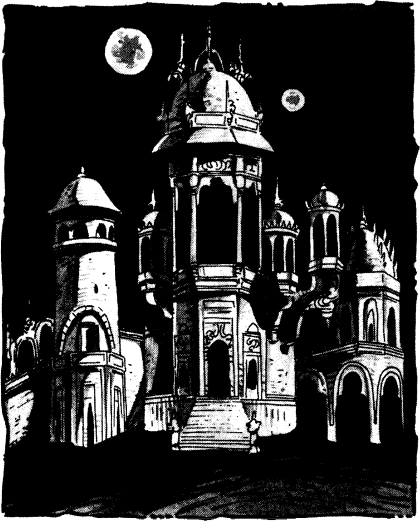
\includegraphics[width=\columnwidth]{images/raam-1.png}
\end{figure}

\City{Raam}
{40,000 (40\% humans, 20\% dwarves, 15\% elves, 10\% muls, 5\% half-elves, 5\% half-giants, 4\% thri-kreen, 1\% other).}
{Silver, gems, flint, jute, silk, textiles.}
{Common, Dwarven, Elven, Raamite.}
{
	Shortly before the day of the Great Earthquake, the sorcerer-queen Abalach-Re was killed in battle with Sadira of Tyr. When the news reached Raam, it was the spark that ignited the fires of anarchy, and now Raam burns. But Raam was a city on the brink of revolution even before the death of its queen. Since Abalach-Re's death, the city has collapsed into chaos. Various factions have grabbed whatever power they could, and Raam teeters on the brink of civil war.
}
{
	Raamish society revolves around a caste system. Each citizen is born into a caste and can never leave it. Members of one caste cannot marry or associate with others from another caste without becoming unclean. Caste and race are not related, and a member of each race can be of any caste.

	The highest caste is made up of priests. This caste includes clerics and druids, as well as teachers, scholars and wise men. Members of this caste wear white garments to distinguish themselves.

	Below the highest caste, is the vizier caste. The templars and soldiers of Abalach-Re fall into this caste. The members of the vizier caste typically wear silk clothing dyed a variety of colors.

	The next caste includes the majority of the nobles of Raam, as well as artisans, and tradesmen. Wealth has no affect on one's caste. The richest tradesmen will never rise above his caste. This caste typically dresses in clothing made of less expensive material than the silk worn by the vizier class.

	The laborers caste is the largest caste and the lowest. It includes all servants and unskilled workers as well as the vast numbers of slaves. Laborer caste members wear simple white linen clothing.

	Below the laborers caste are the truly desperate. Outcastes are those who most handle dead animals and people. Butchers, morticians, and tanners are all included in this caste. They are considered so unclean that they must live outside the city to prevent them from polluting the rest of the citizens.

	The environmental disasters of recent months have had very little impact on Raam. The Great Earthquake was barely perceived, for it caused little damage and no deaths. No Tyr-storm has yet visited the city-state, so Raam's residents have yet to experience the devastation that such a storm can inflict. The death of Abalach-Re and the resulting struggle for power, however, have caused more death and destruction than any force of nature.

	Raam has been divided into armed camps controlled by greedy, power-hungry warlords. Some call themselves templars, others nobles, liberators, or merchant lords. All are raiders and bullies, seeking to use strength as a means of control.

	These armed camps don't even make a pretense of peaceful coexistence. Skirmishes over disputed territories are constantly being fought, as are battles over caches of weapons or supplies-even just to determine which side is stronger! It won't be long before all-out war breaks out to see if one leader and his faction can conquer the others and restore order of some sort to the city. This war, of course, may simply wind up destroying Raam and reducing the verdant belt it occupies to a wasteland.

	Understandably, the free citizens live in a constant state of fear. They have nowhere to go, nowhere to turn to, and conditions within the city become more terrible every day. Some citizens have appealed to one faction or another, offering to become indentured slaves for the protection and sustenance offered by the vying warlords.

	Every day, more and more citizens surrender their freedom in exchange for a safe place to sleep, a cool drink of water, and a bit of food to fill an aching stomach.

	The slaves of the city have fared even worse than the free citizens. Their masters have been replaced by heartless owners who treat the slaves no better than living tools that can be replaced when they break. Some slaves, embracing the legends of Rikus, Neeva, and Sadira of Tyr, have rebelled, using the opportunity presented by the chaos. One group has come under the leadership of a gladiator named Korno (CN male mul, barbarian 1/gladiator 4/arena champion 4). Between Korno's military daring and expertise and the cache of weapons his followers found in one of Abalach-Re's many hidden treasuries, this group of slaves has set itself up as another armed band in a city of gangs. Korno has called for all slaves to join his community, for when they have the numbers to go along with their dreams they will rise up and overthrow all their masters. Korno, however, is as cruel and ruthless as any of the other leaders of the armed bands. The slaves that have flocked to his side continue to be treated as slaves, working to make life easier for Korno and his best warriors.

	With food and water in short supply and violence rampant in the streets, it is little wonder that the people of Raam are turning to anyone or anything that claims to have a solution. In this volatile environment, revolution seems to be inevitable. What the outcome of such an event will be is unknown, but by all indications it will be bloody in the extreme.
}
{
\begin{figure*}[b!]
\centering
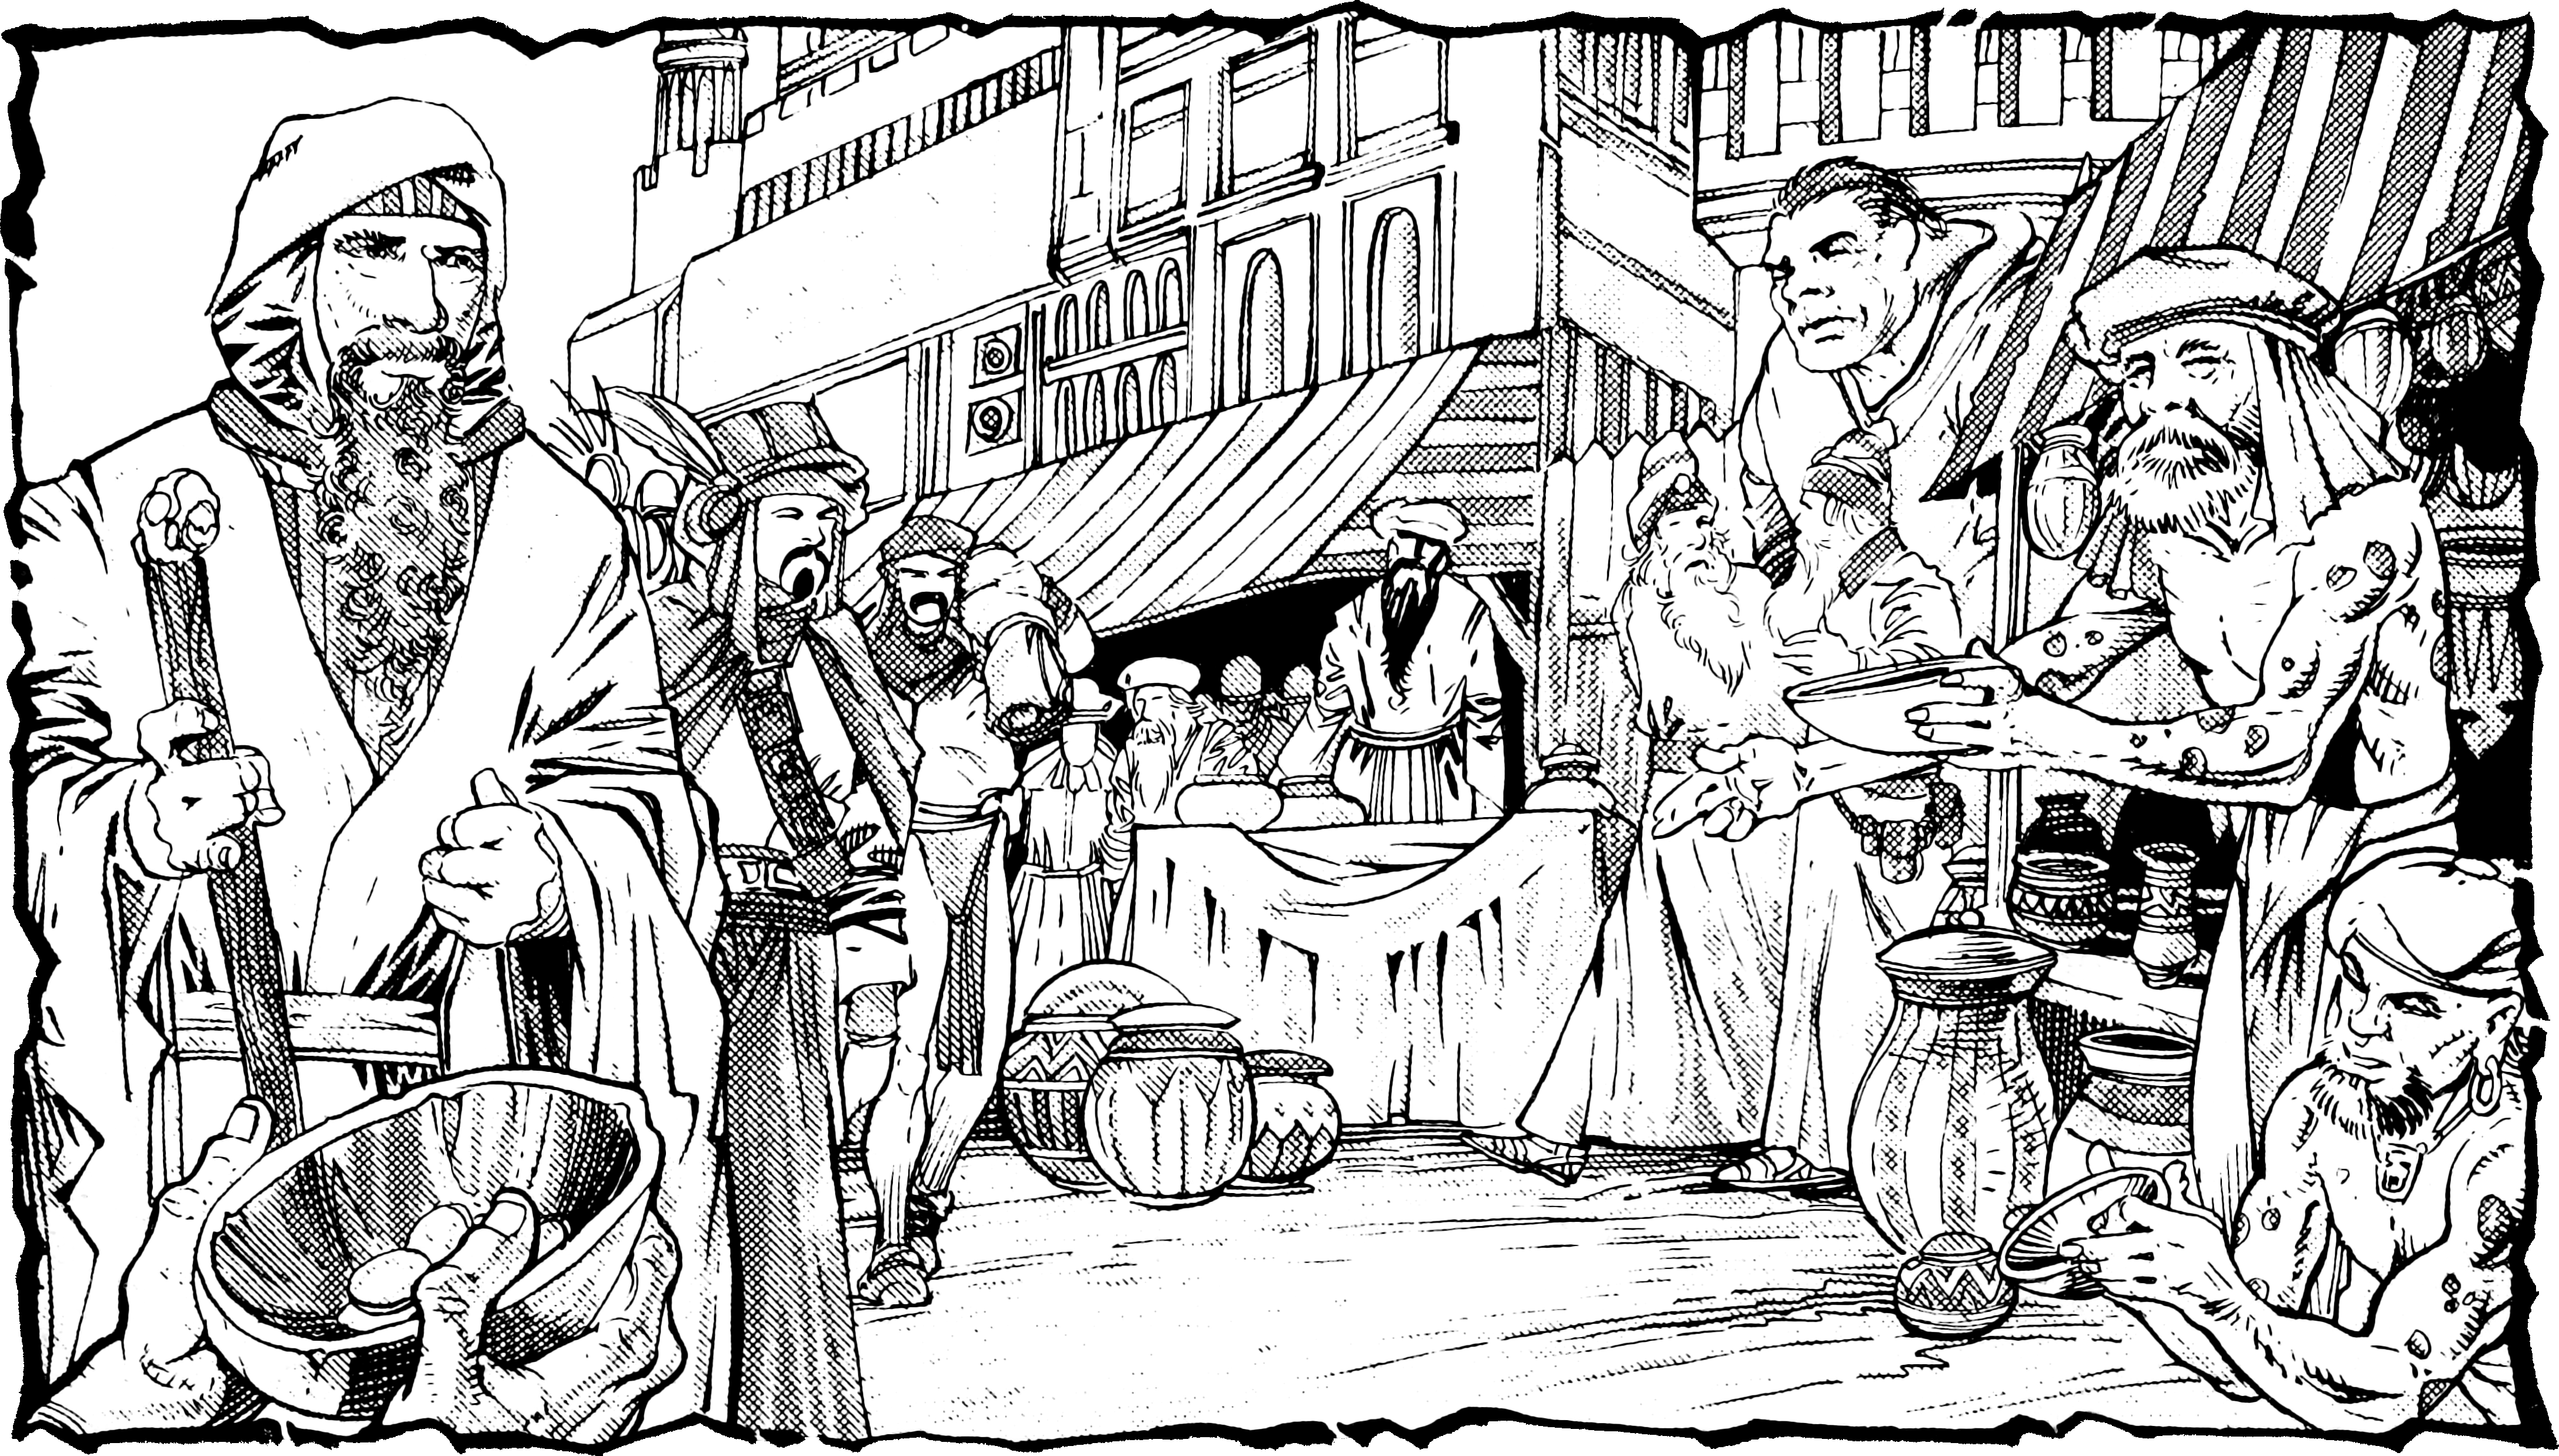
\includegraphics[width=\textwidth]{images/raam-2.png}
\end{figure*}

	The government of Raam still exists, but it has almost no power in the face of the violence and chaos ravaging the city. The templars who haven't fled in fear or tried to hide among the populace as regular citizens continue to administer the city, but it is clear the city no longer functions the way it used to. These templars have only their bureaucratic skills to fall back on, as their ability to use priestly spells vanished with Abalach-Re's demise. The templars continue to call for the worship of Badna, the mysterious (and imaginary) being the sorcerer-queen claimed to receive her powers from. Most people ignore these calls to worship, for they never believed in Badna anyway.
}
{
	\textbf{Leviath the Calm}: Leviath the Calm (LN male half-giant, shaper 9) is an unusual half-giant who speaks of peace and tranquility to all who would listen. His words are spoken with kindness and sincerity, and have had a profound effect on the masses, among which he has developed a large following. Despite his large size and strength Leviath is said to have never raised his voice in anger or struck a blow to harm another living creature.

	\textbf{House M'ke}: The merchant houses have taken one of two tacks regarding conducting business in Raam. The first option, chosen by the vast majority of merchant houses, was to get out of town and take their business elsewhere. The second option, embraced by House M'ke as a prudent enterprise that will ensure its own survival, was to seize control of as much of the city as possible. House M'ke and its army of mercenaries now control most of the merchant district. Armed bands wearing House M'ke's colors periodically sweep through the city, looting and pillaging until they gather enough goods to fill a caravan. This caravan then sets out across the Tablelands to conduct trade as any merchant house caravan would. Only in Raam does House M'ke behave like a conquering army of raiders-because in Raam, that's what House M'ke has become. A few of the more daring (or desperate) merchant houses return to Raam from time to time to test the climate, but they usually wind up losing their goods to one or more of the armed camps seeking dominance in the city.

	\textbf{Night Runners}: The strangest group to stake a claim in Raam's power vacuum is the elf tribe known as the Night Runners. Prior to Abalach-Re's death, the Night Runners maintained a small presence in Raam. Now this group of elves-which specializes in the ``shadow arts'' of espionage, assassination, and extortion-has decided to take a more active role in Raam society. A large portion of the elf quarter and the tradesmen's district has been taken over by the Night Runners. Besides holding and expanding their own territory, the Night Runners continue to sell their unique services to those who can afford them---including noble houses, merchant camps, and even templar domains. In the end, the Night Runners plan to control the entire city, making it the first elf city in thousands of years. Until then, the elves don't mind working for the bands they're competing with, for it gives them an easy way to keep tabs on how the factions are doing.

	\textbf{Nobles}: One of the largest groups claiming dominion over sections of Raam is the noble families. Like the raiding tribes of the sandy wastes, the nobles pillage and plunder for the things they want and need to survive. The nobles have expanded their areas of control. While each family started with a small piece of land and the road adjoining it, those with the power and audacity to press their advantage have grabbed whatever they could hold onto. Like the raiding tribes, the noble camps are savage, ruthless, and have only their own interests at heart.

	\textbf{Prophets of Dregoth}: Strange figures with bizarre accents who hide their features beneath many folds of robes preach of Dregoth the Savior. These prophets claim Dregoth is a god who will bring salvation to Raam if they lay down their weapons and accept him.

	\textbf{Templars}: The main body of templars occupies one camp, centered in the templar quarter of the city. Various rogue templars command smaller parts of Raam, claiming from as little as one building to as many as several blocks as their personal domains. They defend these domains with troops that were once loyal to Abalach-Re but now follow their templar commanders.

	Under Abalach-Re's reign there were two organizations of templars assigned to police the city. The mansabdars were the public force. They were assigned to guard and patrol duties. Though the larger of the two police forces, the mansabdars were corrupt and many were incompetent. The kuotagha was the secret police force. These ruthless enforcers were tasked with administering justice as they saw fit. Disguised as merchants and artisans, they moved freely among the population spying out sedition and unlawful behavior. When they judged someone guilty, the kuotagha executed the suspect without trial, immediately and by surprise. All kuotagha members carried a special garrote called a ghi, for use in such situations.

	\textbf{The Veiled Alliance}: The turbulent conditions in Raam haven't made it any easier for the city's Veiled Alliance. The preservers continue to operate in secret, but the contacts they once had in all levels of government have been lost. Nanda Shatri (LG female human, preserver 7/telepath 4/veiled one 10) continues to lead the Alliance and still seeks to become an avangion so that she can help restore Athas' lost vigor. However, beyond the vague rumors that Urik's Alliance had created such a being some years back, Shatri is no closer to her goal than she was a decade ago. She has considered siding with one of the armed bands in order to assure the safety of her people, but she has yet to determine which band to approach. Her reluctance to make a decision might be her undoing, for the Prophets of Dregoth have begun making overtures to the Alliance that the members find very appealing. In fact, the Prophets have also promised that Dregoth can help Shatri with her research into the avangion transformation process---a promise that she is seriously considering accepting.
}
{
	\textbf{Daro (Thorp, 300)}: Daro was a center of agricultural administration, used to oversee the slaves working the fields of Raam. After the death of Abalach-Re, templar Avish Thira seized control of Daro, instituting martial law which prevented the chaos that swept the rest of the city-state from reaching Daro. Under Avish Thira the village no longer is concerned with agriculture. The fields have been allowed to become fallow and most of the hundreds of field slaves have been freed, actually expelled from the village since Thira could not feed them. Thira supports himself and his guards by sponsoring raids into Raam.
}
{
	\textbf{The Benevolence Center}: The Benevolence Center is the name of a large housing complex for the elderly.

	\textbf{The Consecrated Sepulcher of Badna}: The massive Consecrated Sepulcher of Badna is one of the most majestic buildings in Raam. The Sepulcher is a mausoleum where the remains of the last 30 generations of favorite husbands of sorcerer-queen Abalach-Re were laid to rest.

	\textbf{The Crematory}: The stark granite walls of the Crematory tower over the slums outside the western wall of Raam. There are no windows in the entire building. A large chimney rises from the back of the building, emanating a thick column of smoke. Only outcastes are considered suitable to handle the remains of the dead, and as such the crematory is staffed completely by outcastes. Members of the rest of Raamish society spend as little time as necessary in the Crematory for fear of being contaminated.

	\textbf{The Gallery of the Seven Stars}: The Gallery of the Seven Stars houses the works of Raam's finest sculptures. Built of white rock, the Gallery is decorated with ornate murals and minarets. The museum contains seven star-shaped display halls where magnificent sculptures are displayed.

	\textbf{Natural Arena of Raam}: Raam's gladiator arena is a naturally formed amphitheater formed between two hillocks, outside of the city's walls. Wind and time have carved one of the hillsides into natural seating areas of rust colored rock. The arena floor is a rough oval and has a floor of red sand. A natural crevasse separates the arena floor from the seating area. Known as ``The Maw of Raam'' the chasm runs the full length of the arena floor, and is rumored to be almost 60 meters deep. The bottom of the Maw is difficult to see because of the wild brambleweed that grows within. On the second hillock, the side that forms the back of the arena is a sheer granite wall. The hillock contains many tunnels and secret passages that end at observation spots throughout the hill. It was from here, hidden from the sight of the populace that Abalach-Re and her templars watched gladiator contests.

	\textbf{Psiumarkh}: The Psiumarkh has been the most prestigious of the psionic schools in Raam. It can trace its founding back to the founder of modern psionic principles, Tarandas over 900 years ago. The Psiumarkh has always maintained strict neutrality in the struggles that afflict Raam, allowing them not to anger any of the city's powerful factions.

	\textbf{Royal Barracks}: Located within the Palace district of Raam, near the Ivory Palace, the Royal Barracks is a multi-storey building used as a military barracks for the elite warriors and officers of the Raamish army.

	\textbf{The Ivory Palace}: Abalach-Re ruled Raam from a beautiful palace of ivory and alabaster. Built upon a knoll and surrounded by a series of defensive ditches and walls, Abalach-Re prevented most of her subjects from approaching her palace. Since her fall, various noble factions have attempted to seize and/or loot the palace. Their resulting struggles have destroyed most of the palace. Recently rumors of a curse affecting those who enter the ruined palace are beginning to spread.

	\textbf{Wrestling Pits}: Located near the Elven market, the wrestling pits are used for legal and illegal matches.

	\textbf{The Yellow Monastery}: The Yellow Monastery houses a group of monks who focus their study on telepathic psionic powers. Under the rule of Abalach-Re, the monastery was seen as a symbol of resistance to her rule, as the monks were opposed to slavery as well as the use of magic of any kind. Since the sorcerer-queen's fall, the monks have tried to protect those who live near the monastery against the chaos that has engulfed the city, but to little effect. They are rumored to have befriended the half-giant Leviath the Calm and his followers.
}
{
	\item An undead war beetle is no longer under the control of its handlers and goes on a rampage. Something has wrestled control of the beast away from its handlers and the PCs must board the undead war machine and face whatever it is.
	\item The situation in Raam is getting desperate. One morning a large group of members of the laborer caste gathers in front of the PCs' dwelling. Desperate for food, they believe the PCs are hoarding food. After building up their courage, the rioters attack the dwelling. The rioters are lead by a deranged woman who clutches the undernourished body of a small baby. In her desperation, the woman deludes herself into thinking the baby is still alive. Even if the PCs drive off the rioters, rumors of their hoard of food spread quickly around the city. Other more powerful forces, such as templars and nobles, seek to gain the PCs hidden food hoard for themselves.
	\item The forces of the t'liz, Nevarli (see Terrors Beyond Tyr for more information), invade a client village near Raam. She intends to use the village as a base for her invasion of Raam, as well as using the villagers as her feeding stock. Nevarli's forces include undead, humanoids, and other-planar creatures.
	\item In the chaos after news of Queen Abalach-Re's death reached the city many attempted to loot the Queen's palace. Most of the looters were disappointed because the Queen's treasury was never found. Rumors say the queen hid her treasury but the location varies with each telling. Some say the Royal Barracks, others underneath the Gallery of the Seven Stars, and many claim the treasure is hidden with Abalach-Re's former husbands in the Sepulcher of Badna.
	\item A salt golem built by Sorcerer-Queen Abalach-Re stood unmoving guard over a fountain in her palace until her death. Without warning, the creature has struck out into the city traveling from one public well to the next, attacking anyone it sees gathering water from the wells. The PCs may seek to destroy the creature but some templars want to capture the creature and figure out a way to gain control over it.
	\item The gem mines south of Raam have been abandoned for years. Recent reports say that undead have been sighted around the mine. The undead do not attack those who maintain their distance but killed and devoured a group of elves that tried to enter the mine.
}